\documentclass[12pts]{report}

\usepackage[margin=1in]{geometry}
\usepackage[usenames, dvipsnames]{color}
\usepackage{setspace}
\usepackage{graphicx}
\doublespacing
\usepackage{fancyvrb}
\usepackage{varwidth}
\usepackage{verbatim}
\usepackage{multicol}
\usepackage{float}
\usepackage{fancyhdr}
\usepackage{parskip}    % This packages sets the spacing between two paragraphsc   
\usepackage{hyperref}              
\setlength{\parskip}{.5\baselineskip}   % Define spacing between two paragraphs

\setlength{\parindent}{0pt}
\setlength{\columnseprule}{0pt}

\pagestyle{fancy}
% Title Page
\title{DIME DYNAMIC DOCUMENTATION TRAINING \\ Exercise 2}
\author{Luiza Andrade \& Mrijan Rimal} 
\date{\today}

\fancyfoot{}
%\fancyhead[C]{\thepage}
\cfoot{\small{For the most recent version of the file, please check \url{https://github.com/worldbank/DIME-LaTeX-Templates/} } \\ \thepage}

\makeatother


\begin{document}
	
	
	\makeatletter
	\begin{titlepage}
		\begin{center}
			
\includegraphics[width=0.3\linewidth]{../img/i2i.png}\\[10ex]
			{\LARGE \bfseries  \@title }\\[2ex] 
			{\Large  \@author}\\[20ex] 
			{\large \@date}
		\end{center}
	\end{titlepage}
	\makeatother
	
\section*{Introduction}
Exercise 1 introduced you to the basics of how to import tables and figures to a {\LaTeX} document. This exercise will introduce you to some intermediate topics commonly used to make your document look even more professional.

We will also show how {\LaTeX} can be used to create a dynamic document that updates automatically once your output from, for example, Stata or R is updated without any error prone manual copy-and-pasting.

 

\section*{Part 1. Exporting tables}
In this section, you have the option of using the template do file provided in \textcolor{red}{Dynamic-Documentation/Exercises/Stata Export Exercise/Export tables and images.do} to export graphs and figures OR using your own data and generating tables and graphs that can be imported into {\LaTeX}. 

If you're using the do file provided, change the folder paths in the do file to your directory structure and run the do-file. This will export two tables and two graphs to the Raw folder that will be used in the exercises that follow.  

If you would like to work with your own data, please follow the following steps. 

\begin{itemize}
	\item Make sure that you export \textbf{two tables} and \textbf{two graphs} using your own data. For help, you can look at the folder called ``Exercise Stata - How to export tables and graph from Stata to LaTeX''.
	\item Make sure that all the exporting is done using Stata do-files, or R scripts so you can easily export them again by just running the code. Towards the end of this exercise we will ask you to make changes to your do-file or R script so if you are using a file from an actual project you may want to make a copy of your do-file or R script that you can use in this exercise.
	\item Import all the tables and figures you have created in step 1 into your {\LaTeX} document. Sample code to import tables and figures can be found in the \textbf{DIME Templates} sub-folder. Make sure to use the  code in \texttt{Template 1 - Importing tables.tex} file to import figures(not tables), and the code in \texttt{Template 2 - Importing figures.tex} file template to import graphs(not tables). It will not work if it is the other way around.
	\item Make sure you give a caption to your tables. 
\end{itemize}

\section*{Part 2. Intermediate {\LaTeX} Exercises}
\subsection*{Part 2.1 Adding Sections to your document}
{\LaTeX} automatically formats the document and different section headers and subheaders according to predefined formats. It also allows you to automatically create a beautiful \texttt{Table of Contents} based on what has been defined as sections and subsections. 

Sections can be created using \verb|\section{title}| command. {\LaTeX} automatically numbers all the sections in the order you put them. Since, you manually don't specify chapter and section numbers, you can cut and paste subsections from the end to the beginning and the numbering will update automatically! 

Similarly, subsections can be created using \verb|\subsection{title}| and sub-sub-sections can be created using \verb|\subsubsection{title}|. The subsections will be numbered on the format 1.1 and the subsubsection will be numbered on the format 1.1.1. An example is shown in Annex 1\ref{sec:Annex}. 

\textit{Note: Sections and subsections can be created using} \verb|\section*{title}| \textit{if you do not want your sections numbered in the document. However, these sections and subsections will not be shown in the table of contents.}


\clearpage
\subsection*{Part 2.2. Adding Table of Contents}

After we have set up sections, sub-sections and sub-sub-sections you can easily add a table of contents to your {\LaTeX} document by using \verb|\tableofcontents| in your docuemnt. You can create this any where you want, but typically this is created directly after \verb|\begin{document}| or after \verb|\maketitle| if you have a title.  An example is shown below:

\begin{Verbatim}[commandchars=+\(\)]
	\documentclass[12pts]{article}
	
	\title{My Awesome Document}
	\author{John Doe}
	
	\begin{document}
	\maketitle
	+color(CornflowerBlue)\tableofcontents
	\newpage

\end{Verbatim}
The above {\LaTeX} code is used to generate table of contents below.

\begin{figure} [H]
	\centering
	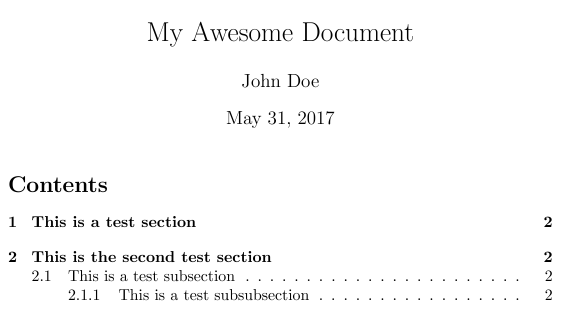
\includegraphics[width=.8\linewidth]{../img/tableofcontents2}
	\caption{Example table of contents generated from our document in Annex 1.}
	\label{fig:tableofcontents}
\end{figure}

\subsection*{Part 2.3. Referring to your tables, and figures in a document}

Just like the numbering of sectiona and sub-sections, {\LaTeX} uses a dynamic referencing system for tables and figures etc. In the text in your docuemnt where you describe your tables and figures you are likely to want to refer to them on a format similar to "\textit{As you can see in figure 2...}". Since the numbering of tables and figures is updated automatically, you need a way for your references in your text to be updated automatically as well.

In {\LaTeX} that is solved by giving tables and graphs a unique name using the \verb|\label{}| command. In the text where you want to reference a figure or a table, you reference the name used in the label and {\LaTeX} will update the numbering for you as your documents grows and changes.

The labels are categorized into the type of item you are referencing, so you label tables and figures slightly differntly. We will show how it is done in the following sub-sections.

\subsubsection*{Part 2.3.1 Referring to Figures in a document}
To refer to figures, we will use the \verb|\label{fig:figurename}| command. Inside the brackets in the \verb|\label{}| command you see two parts seperated by a colon. The first part  \texttt{fig} indicates that this is a figure that we are assigning a label to. The second part  \texttt{figurename}, you should replace with the unique name you want to use to refer to this figure.
  
We must add the \verb|\label{fig:Figurename}| line inside the \verb|\begin{figure}| and \verb|\end{figure}| in our codes. See below:

\begin{Verbatim}[commandchars=+\(\)]
	\begin{figure}[H]
	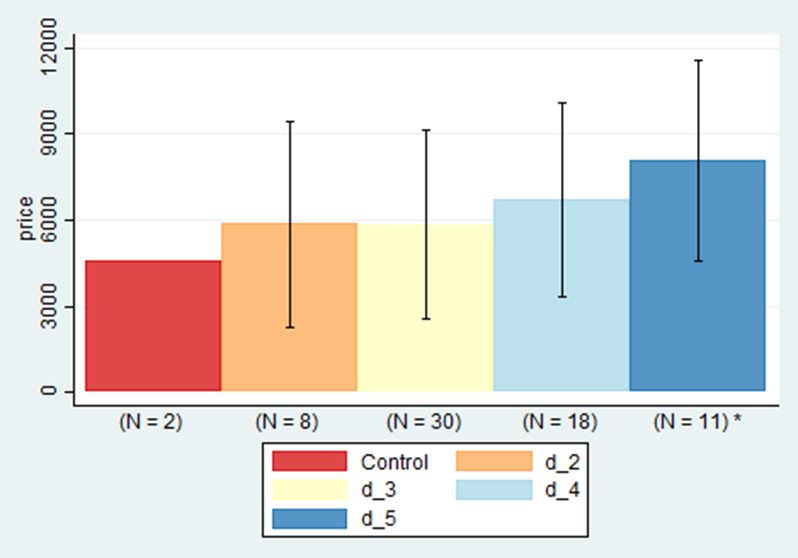
\includegraphics[width=\textwidth]{../Raw/iegraph.png}
	\caption{Add figure title here}
	+color(CornflowerBlue)\label{fig:iegraph}
	\end{figure}
\end{Verbatim}

Now to refer to the figure anywhere in the document, you can type \verb|\ref{fig:iegraph}| and it will automatically refer to the figure using the correct number in the document. In our example, if the \texttt{iegraph}	figure is the fourth one in the document, \verb|As you can see in figure \ref{fig:iegraph}| will appear as \texttt{As you can see in figure 4,} in the document. 

\subsubsection*{Part 2.3.2 Referring to Tables in a document}

Similarly for tables, we can also refer to them anywhere in the document using the same method. To refer to tables, we will use \verb|\label{tab:tablename}| command inside our \verb|\begin{table}| and \verb|\end{table}| like the example below. 

First, we need to add a label to the table that has been imported to the document by adding \verb|\label{tab:tablename}| inside the \texttt{begin} and \texttt{end} table in our code. 

\begin{Verbatim}[commandchars=+\(\)]
	\begin{table}[H]
	\caption{Add a title to this table}
	{
\def\sym#1{\ifmmode^{#1}\else\(^{#1}\)\fi}
\begin{tabular}{l*{4}{c}}
\hline\hline
          &\multicolumn{1}{c}{Group 1}&\multicolumn{1}{c}{Group 2}&\multicolumn{1}{c}{Group 3}&\multicolumn{1}{c}{Group 4}\\
\hline
Control   &       203         &       945         &        700         &        200         \\
Treatment &       151         &       952         &        952         &        148         \\
\hline
Total     &       354         &       1897         &       1652         &       348         \\
\hline\hline
\end{tabular}
}

	+color(CornflowerBlue)\label{tab:samplesize}
	\end{table}
\end{Verbatim}

Now we can refer to the above table in our document by typing \verb|\ref{tab:samplesize}| which will automatically refer to the table using the correct number in the text in your document. 

\subsection*{Part 2.4 Text Formatting}

Now that you have created sections in your document, and added text, you might want to change some of the formatting of your text. In {\LaTeX} you are formatting your text using packages and code. We will here include a few topics.

\subsubsection*{Part 2.4.1 Bold, italic and underlined}

\subsubsection*{Part 2.4.2 Color}

\subsubsection*{Part 2.4.3 Line Spacing}
Now that you have created sections in your document, and added text, you might want to change the spacing between lines. This can be achieved using the \texttt{setspace} package. 

The steps to change line spacing are as follows:
\begin{itemize}
	\item Before \verb|\begin{document}|, declare the package you will be using. In this case, \verb|\usepackage{setspace}|. This package controls the line spacing in a {\LaTeX} document.
	\item After using the \texttt{setspace} package, you should now specify line spacing which are as follows:
	\begin{description}
		\item[singlespacing] This option specifies the document to use one line spacing.
		\item[doublespacing] This option specifies the document to use two line spacing.
		\item[onehalfspacing] This option specifies the document to use one and a half line spacing. 
	\end{description}
\end{itemize}
\begin{Verbatim}[commandchars=+\(\)]
+color(CornflowerBlue)\usepackage{setspace}
+color(CornflowerBlue)\doublespacing
+color(Gray)%\onehalfspacing
+color(Gray)%\singlespacing
\begin{document}
\maketitle
\listoftables
\listoffigures
\section{Introduction}
This is the introduction paragraph
\end{Verbatim}
The \texttt{setspace} package can also be used to specify more particular linespacing i.e. 1.7 lines, 2.4 lines etc using the \texttt{setstretch} feature but that will be covered in another documents. 

\subsection*{Part 2.5. Rotating a table landscape}

Sometimes the tables are very wide and need to be in landscape format. This can be adjusted using the \texttt{adjustbox} package which we have been using for importing tables. 

\begin{Verbatim}
\begin{table}[H]
	\caption{Add table title}
	{
\def\sym#1{\ifmmode^{#1}\else\(^{#1}\)\fi}
\begin{tabular}{l*{4}{c}}
\hline\hline
          &\multicolumn{1}{c}{Group 1}&\multicolumn{1}{c}{Group 2}&\multicolumn{1}{c}{Group 3}&\multicolumn{1}{c}{Group 4}\\
\hline
Control   &       203         &       945         &        700         &        200         \\
Treatment &       151         &       952         &        952         &        148         \\
\hline
Total     &       354         &       1897         &       1652         &       348         \\
\hline\hline
\end{tabular}
}

	\label{tab:samplesize}
\end{table}
\end{Verbatim}
To rotate the table to landscape, we can use the \texttt{adjustbox} feature with the \texttt{angle = 90} option as shown in blue in the code below.
\begin{Verbatim}[commandchars=+\(\)]
\begin{table}[H]
	\caption{Add table title}
+color(CornflowerBlue)	\begin{adjustbox}{angle = 90} 
		{
\def\sym#1{\ifmmode^{#1}\else\(^{#1}\)\fi}
\begin{tabular}{l*{4}{c}}
\hline\hline
          &\multicolumn{1}{c}{Group 1}&\multicolumn{1}{c}{Group 2}&\multicolumn{1}{c}{Group 3}&\multicolumn{1}{c}{Group 4}\\
\hline
Control   &       203         &       945         &        700         &        200         \\
Treatment &       151         &       952         &        952         &        148         \\
\hline
Total     &       354         &       1897         &       1652         &       348         \\
\hline\hline
\end{tabular}
}

+color(CornflowerBlue)	\end{adjustbox}
\label{tab:samplesize}
\end{table}
\end{Verbatim}

This will rotate the table to the specified degree in the final document. 

\section*{Part 3. Making a Dynamic Document}

Here, we will produce a dynamic document. Please only do this do \textbf{if} you have completed up to \texttt{Part 2.5} of this exercise document. 

\begin{enumerate}
	\item Generate a pdf document by compiling the document and save the pdf created up to now in a separate location from the \texttt{.tex} document where you have input the codes to import the tables and graphs. 
	\item Generate a new treatment for your dataset by dropping a subset of your data set. 
	\subitem If you are using the Stata do-file template provided in the Dynamic Documentation Folder, then only keep observations from Europe and Central Asia, and drop observations from North America and South America. This can be done by using the Stata codes \texttt{drop if region!= 1}. 
	\item Rerun the do-file . Make sure that the tables and graphs you created earlier are overwritten i.e. save them without updating any paths so they save and replace the tables and graphs created earlier. 
	\item Now, open the {\LaTeX} file\footnote{The one where you imported all your graphs and figures.} you created earlier and press \textit{Build and Compile} under the \textit{Tools}.
	\item Now if you compare the pdf file you have just generated with you new data with the one you saved earlier, you will find that the tables would have updated automatically. 
\end{enumerate}

\section*{Part 4. Challenge: Using a do-file to edit a .tex file after exporting it}
\textit{Note: This is an advanced exercise and you don't have to feel compelled to finish it. This is also best done after finishing all the other exercises in the GitHub repository.}
 
During this part of the exercise, you will learn how to use commands in Stata to format your tables. The reason for doing this is that we want to make as little edits in {\LaTeX} as possible, so that when we update the tables like we did in Part 3, everything in the document file updates automatically. So, we would want to tweak or format our tables automatically using Stata, so that we do as little work in {\LaTeX} as possible.

While tables exported from Stata to {\LaTeX} are generally very nice, sometimes they need to be tweaked a little to make them look nicer. So, in this exercise, we'll use the \texttt{filefilter} command in Stata to make small changes to the files exported by Stata. \texttt{filefilter} is one such command in Stata which used to edit output files generated by Stata.  

This exercise requires more familiarity with {\LaTeX} than previous exercises. Don't worry if you can't complete it. 

\begin{description}
	\item[Task 1:] Run the initial code for exercise 6 in the \textcolor{red}{Add path and name of do-file} do-file. This will create a table with sample sizes for control and treatment groups across regions and in the whole sample. Add this table to the .tex file you created in the Exercise 2, Part 1. How does that look?
	\item[Task 2:] Open the \textcolor{red}{Dynamic-Documentation/Exercises/Exercise 1/Output/Raw/sample\_sizes.tex} file created by Stata. Can you identify the source of the extra spacing?
	\item[Task 3:] Use the \texttt{filefilter} command in Stata to filter out the lines or characters in the fragmented file that create the extra spacing. Import the new .tex file and check how it looks.
	\item[Task 4:] Repeat task 3 if necessary.
\end{description}


\newpage
\section*{Annex 1 : Creating sections}
\label{sec:Annex}
\begin{figure}[H]
	\centering
	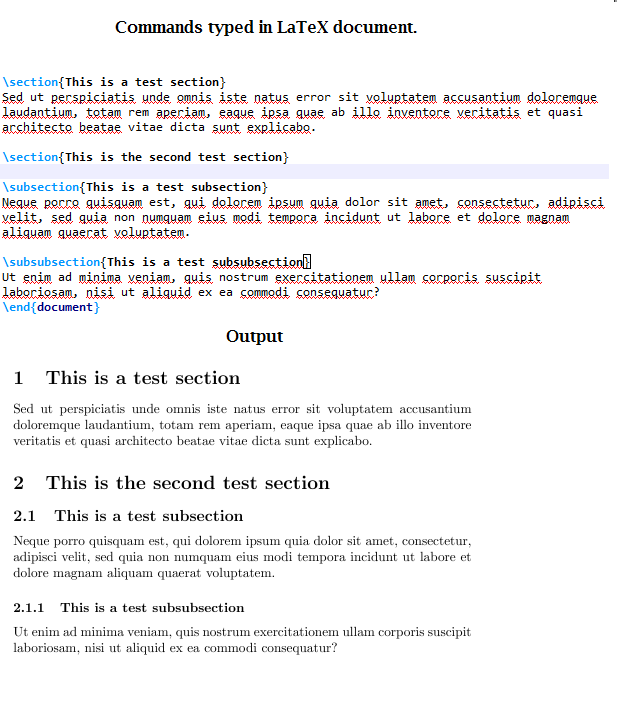
\includegraphics[width=0.7\linewidth]{../img/section}
	\caption{Adding sections and subsections in a {\LaTeX} document}
	\label{fig:adding sections}
\end{figure}
\end{document}          
